
%%%%%%%%%%%%%%%%%%%%%%%InSTA2015の論文
\chapter{I/O テストデータパターンによるテストケース抽出手法}\label{chap:4}
本章では,テスト分析において,テスト条件を網羅的に特定する方法として,テスト実行時のデータの入出力(以降I/Oと呼ぶ)に着目する.
テストベースを分析する際に,テスト実行時のI/Oの要素で分析を進めることで,網羅的にテスト条件を特定する方法としてI/Oテストデータパターンを提案する.
3章の題材を使って提案手法の適用評価を行う.
また,現実に使われたモバイルアプリケーション開発プロジェクトのテストケースを入手し,そのテストケースとI/Oテストデータパターンを使って特定したテスト条件の内容を比較し,手法を適用することで特定できるテスト条件にどのようなものがあるかを確認する.

\newpage
\section{I/Oテストデータパターンの概要} \label{sec:4-1}
\subsection{テストカテゴリベースドテストの課題} \label{sec:4-1-1}
3章で示した予備実験を通して,テストカテゴリベースドテストの適用に一定の効果は確認できたものの,テストカテゴリベースドテストの知識を与えるだけでは,期待した数のテスト条件を特定できないことを確認した.
また,業務経歴3年未満の技術者には有効であったが,3年以上の技術者には効果を観察できなかった.
テストカテゴリベースドテストは,テストベースの分析に論理的機能構造を基にしたテストカテゴリをガイドとして使用することを明示しているだけであり,具体的な分析手順について定義できていないことが理由だと考えられる.

\subsection{I/Oテストデータパターン} \label{sec:4-1-1}
テストを実行するためには,テスト対象となる$AS$のタスク$Ta$に対して,源泉$So$からデータを入力し,$Ta$から$So$へ出力されたデータと期待結果とを比較する.

たとえば,シンプルな機能の四則演算の計算結果が正しいことを検証するときには,$AS$の外部となる源泉$So_i$から計算の対象となる複数の値$In_i$を入力し,タスク$Ta_i$がそれらの値を計算し,計算結果$Out_i$をテスト対象の外部である$So_i$へ出力する.

これは図~\ref{fig:D-3-Fig4}で示している「外部からのデータ入力,外部へのデータ出力」というパターンになる.また,$So_j$から入力する数値$In_j$に対して,保持データ$Ds_j$である固定比率を使って計算を行う場合,$Ta_j$は$Ds_j$を呼び出し,計算にその値を利用してから計算結果$Out_j$を$So_j$へ出力する.
これは図~\ref{fig:D-3-Fig4}で示している例「外部と内部からのデータ入力,外部へのデータ出力」となる.

\begin{figure}[htbp]
 \begin{center}
 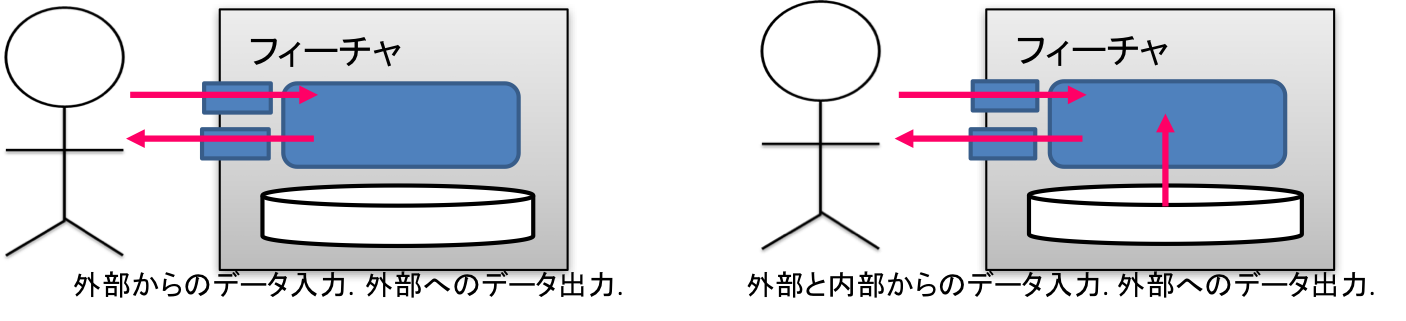
\includegraphics[width=12cm]{./image/D-3-Fig4.png}
 \caption{テスト対象へのデータ入出力の説明}
 \label{fig:D-3-Fig4}
 \end{center}
\end{figure}

テスト実行をするときの$Ta$へのデータ$In$のパターンは,外部からの入力,内部に保持したデータの入力,外部と内部からの入力の3パターンに分類できる.
同じようにテスト対象からのデータ$Out$のパターンは外部への出力,内部に保持したデータの出力,外部と内部からデータの出力の3パターンに分類できる.
これらテスト対象に対するテスト実行時のデータの入出力をまとめたパターンは図~\ref{fig:D-4-Fig6}のように9パターンに集約できる.

\begin{figure}[htbp]
\begin{center}
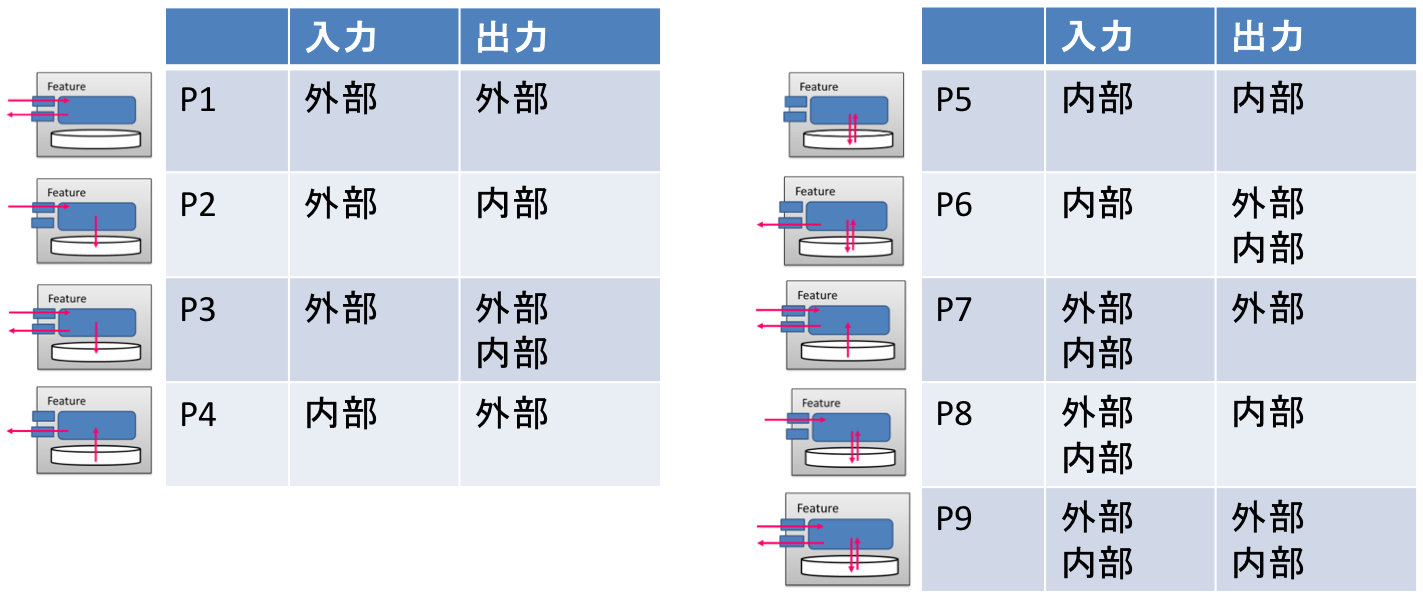
\includegraphics[width=14cm]{./image/D-3-Fig5.png}
\caption{I/Oテストデータパターン}
\label{fig:D-4-Fig6}
\end{center}
\end{figure}

これをI/Oテストデータパターンと呼ぶ\cite{yumoto2015IPA}.
I/Oテストデータパターンがテスト実行時のデータの入出力から見た全体集合となる.

Whittakerによって提案されているフォールトモデル\cite{whittaker2003break}は,$AS$の$Ta$に対する$In$と$Out$のモデルに関する類似の研究である.
フォールトモデルの目的はフォールトを見つけることであり,I/Oテストデータパターンで提示しているデータの入出力モデルはテストベースからテスト条件の中の仕様項目を特定するためのモデルとして使われる.

注意すべきこととしてI/Oテストデータパターンはテスト対象の外部からの観察が可能なものを選ぶことがあげられる.
$Ta$の起動終了に使われる内部のコマンド(シグナルやイベント)は,I/Oテストデータパターンとしては考慮しない.
なぜなら,この手法はブラックボックステストのためのテストベースの分析手法であり,$AS$内部のシグナルやイベントのような外部観察ができないコマンドは,システムテストレベルでのブラックボックステストでは,明示的に考慮できないからである.

テスト分析で特定した仕様項目は,テスト実行をした際の入出力にて確認することができなければならないので,すべてが9パターンのどれかに分類できると考えられる.

\subsection{テストカテゴリベースドテストとの関係}

P1からP9のI/Oテストデータパターンは,単一の$Ta$に対するデータ入出力の全体像となる.
テスト実行の際,$So$から入力を行い,$So$へ出力する間に,データは,テスト対象となる$Ta$によって論理的機能構造の入力調整,出力調整,変換,貯蔵を通過する.
I/OテストデータパターンのP1からP9のそれぞれが論理的機能構造のどの要素に該当するかを表~\ref{tab:D-4-tab1}にまとめた.

% Table generated by Excel2LaTeX from sheet 'Sheet3'
\begin{table}[htbp]
  \centering
  \caption{I/Oテストデータパターンと論理的機能構造}
    \begin{tabular}{|r|p{3em}|l|l|l|p{4em}|l|l|}
    \hline
          & \multicolumn{1}{l|}{} & \multicolumn{1}{p{4em}|}{入力調整} & \multicolumn{1}{p{4em}|}{出力調整} & \multicolumn{1}{p{2em}|}{変換} & 貯蔵 & \multicolumn{1}{p{4em}|}{サポート} & \multicolumn{1}{p{4em}|}{相互作用} \bigstrut\\
    \hline
    \hline
    \multicolumn{1}{|p{1.5em}|}{入力} & 外部 & \multicolumn{1}{p{4em}|}{P1,P2,P3} &       & \multicolumn{1}{p{4em}|}{P1,P2,P3} & \multicolumn{1}{l|}{} &       &  \bigstrut\\
\cline{2-8}          & 内部 &       &       & \multicolumn{1}{p{4em}|}{P4,P5,P6} & P4,P5,P6 &       &  \bigstrut\\
\cline{2-8}          & 外部と内部 & \multicolumn{1}{p{4em}|}{P7,P8,P9} &       & \multicolumn{1}{p{4em}|}{P7,P8,P9} & P7,P8,P9 &       &  \bigstrut\\
    \hline
    \multicolumn{1}{|p{1.5em}|}{出力} & 外部 &       & \multicolumn{1}{p{4em}|}{P1,P4,P7} &       & \multicolumn{1}{l|}{} &       &  \bigstrut\\
\cline{2-8}          & 内部 &       &       &       & \multicolumn{1}{p{4em}|}{P2,P5,P8} &       &  \bigstrut\\
\cline{2-8}          & 外部と内部 &       & \multicolumn{1}{p{4em}|}{P3,P6,P9} &       & \multicolumn{1}{p{4em}|}{P3,P6,P9} &       &  \bigstrut\\
    \hline
    \end{tabular}%
  \label{tab:D-4-tab1}%
\end{table}%


P1に分類できるシンプルな四則演算を行う$Ta$の場合,外部からの入力に対して外部に出力する間に,
図~\ref{fig:D-4-Fig7}のように論理的機能構造の入力調整,変換,出力調整を通過する.
そのため,P1は,表~\ref{tab:D-4-tab1}の以下の3箇所にプロットされている.
\begin{itemize}
  \item 列:入力調整 行:入力/外部
  \item 列:出力調整 行:出力/外部
  \item 列:変換 行:入力/外部
\end{itemize}

このデータフローで通過する3箇所が,P1の場合の期待結果を確認する候補となる.
これらを本研究ではチェックポイントと呼ぶ.
チェックポイントのうち,期待結果を意図的に確認する必要があると判断したものがテスト分析で特定すべき仕様項目,つまりテスト条件となる.

 \begin{figure}[htbp]
 \begin{center}
 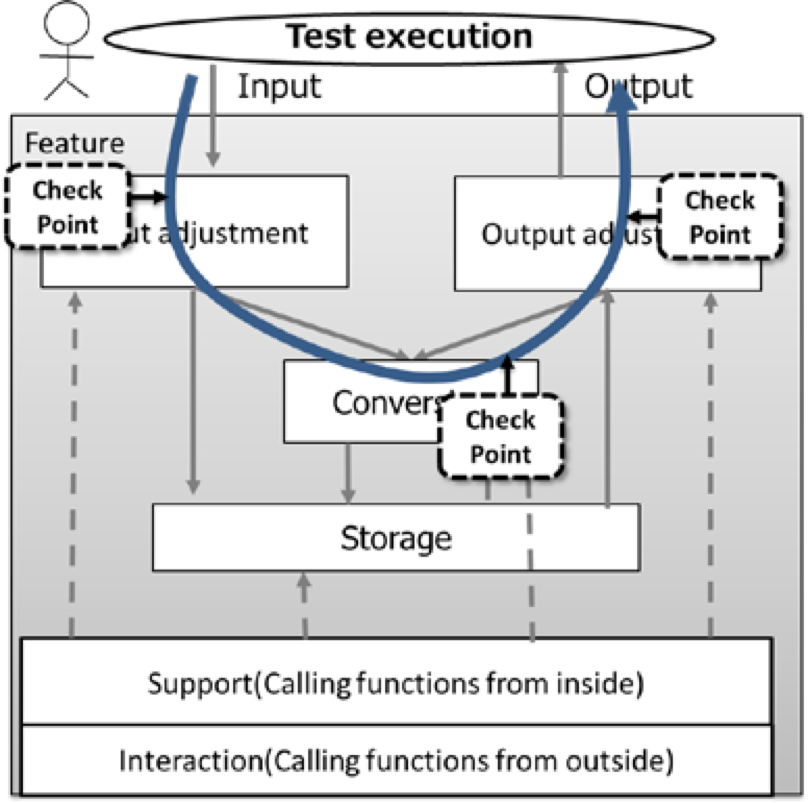
\includegraphics[width=10cm]{./image/D-4-Fig7.png}
 \caption{I/Oテストデータパターンのデータの流れ}
 \label{fig:D-4-Fig7}
 \end{center}
 \end{figure}

データフローの中で通過する3箇所のチェックポイントのうち,少なくとも1つのチェックポイントをテスト条件として特定するが,全てが実際に期待結果を確認する仕様項目になるとは限らない.
例えば,テストすべき仕様項目を特定する際に,入力調整に該当する入力の際に適切な値だけ受け入れることと,変換に該当する計算が適切に行われていることはテストすべきであるが,出力調整が適切にされることは,すでに自明であるためにテストケースとする必要がないということが考えられるためである.

また,表~\ref{tab:D-4-tab1}では,サポートと相互作用についてはデータパターンがプロットされていない.
P1からP9のI/Oテストデータパターンは,単一の$Ta$に対するデータ入出力の全体像だからである.
論理的機能構造の要素である入力調整,出力調整,変換,貯蔵は,外部観察可能な単一の$Ta$に対するデータ入出力のみを考慮している分類であるのに対して,サポートと相互作用は,単一の$Ta$に対するデータ入出力だけではなく,関係する他の$Ta$の呼び出しに着目して仕様項目を特定するための分類である.

サポートと相互作用に分類される仕様項目は,単一の$Ta$に対するデータの入出力の後,何かしらの方法で呼び出した他の$Ta$の出力で期待結果を確認する.
呼び出されたタスクのI/Oテストデータパターンは,論理的に全パターンが発生する可能性がある.


\newpage
\section{I/Oテストデータパターンの適用評価}
本節では,I/Oテストデータパターンの考え方を,3章で行なったテストカテゴリベースドテストの知識を与える前と後を比較する実験結果を使って適用評価を行う.
最初に,演習にて利用したテスト分析の講師解答例をI/Oテストデータパターンに分類するために,解答例のテスト条件に対して,P1からP9の識別子を属性として付与する.
そして,「3.2節 グループ単位の検証実験からの考察」での実験結果を3章の表~\ref{tab:D-3-tab4}で示した評価レベルで整理する.その後,表~\ref{tab:D-4-tab1}と同じフォーマットの表に出現結果を当てはめて,これらの題材にてどのI/Oテストデータパターンが現れるのかを確認する.

\subsection{論理的機能構造の適用評価の分析}
グループ単位の検証実験からの考察では,ヘッドセットのフィーチャセットであるボリュームコントロールと,フライト予約システムのフィーチャセットである新規フライト予約の2種類の異なった題材を実験に使用した.
この実験では,被験者のグループがテストカテゴリベースドテストの知識を得ることでテスト条件をどのように多く特定できるようになるかを確認している.
この実験結果をI/Oテストデータパターンにて評価した結果は,表~\ref{tab:D-4-tab7}と表~\ref{tab:D-4-tab8}に示したとおりである.
前節の結果と本節の結果では行数が異なる理由は, 同じテストカテゴリに属する仕様項目だとしてもデータの入出力が異なるものがあり,場合によってはI/Oテストデータパターンを付与していることがあるためである.例えば,表~\ref{tab:D-4-tab7}では,変換が2行あるが,I/OテストデータパターンはP4とP1となることが該当する.
この実験結果からは,表~\ref{tab:D-4-tab7}と表~\ref{tab:D-4-tab8}が示すとおり, P1, P2, P4, P7 がフィーチャセットに対応するI/Oテストデータパターンとなる.

% Table generated by Excel2LaTeX from sheet 'データの入出力ごとフェリカ (掲載用加工)'
\begin{table}[htbp]
  \centering
\caption{音楽再生機器の演習結果とI/Oテストデータパターン}
    \begin{tabular}{|l|l|l|l|l|l|l|l|}
    \hline
    \multicolumn{2}{|c|}{\multirow{2}[4]{*}{論理的機能構造}} & \multicolumn{6}{c|}{グループ} \bigstrut\\
\cline{3-8}    \multicolumn{2}{|c|}{} & TM1   & TM2   & TM3   & TM4   & TM5   & TM6 \bigstrut\\
    \hline
    \hline
    変換 & P4    & B     & B     & B     & B     & -     & B \bigstrut\\
    \hline
    変換 & P1    & B     & A${}^\text{+}$    & B     & B     & B     & - \bigstrut\\
    \hline
    出力 & P7    & -     & -     & -     & -     & -     & A${}^\text{+}$ \bigstrut\\
    \hline
    貯蔵 & P2    & -     & A${}^\text{+}$    & -     & A${}^\text{+}$    & A${}^\text{+}$    & - \bigstrut\\
    \hline
    サポート & P1    & B     & B     & B     & B     & B     & B \bigstrut\\
    \hline
    相互作用 & P1    & B     & A${}^\text{+}$    & A${}^\text{+}$    & A${}^\text{+}$    & A${}^\text{+}$    & A${}^\text{+}$ \bigstrut\\
    \hline
    相互作用 & P4    & B     & B     & B     & A${}^\text{+}$    & B     & A${}^\text{+}$ \bigstrut\\
    \hline
    \end{tabular}%
\label{tab:D-4-tab7}%
\end{table}%

% Table generated by Excel2LaTeX from sheet 'D論4章用'
\begin{table}[htbp]
  \centering
\caption{フライト予約システムの演習結果とI/Oテストデータパターン}
    \begin{tabular}{|l|l|l|l|}
    \hline
    \multicolumn{2}{|c|}{\multirow{2}[4]{*}{論理的機能構造}} & \multicolumn{2}{c|}{グループ} \bigstrut\\
\cline{3-4}    \multicolumn{2}{|c|}{} & TM1   & TM2 \bigstrut\\
    \hline
    \hline
    変換 & P7    & A     & A \bigstrut\\
    \hline
    入力 & P1    & B     & B \bigstrut\\
    \hline
    入力 & P7    & A     & - \bigstrut\\
    \hline
    入力 & P4    & -     & - \bigstrut\\
    \hline
    出力 & P4    & B     & B \bigstrut\\
    \hline
    出力 & P4    & A     & A \bigstrut\\
    \hline
    出力 & P7    & B     & B \bigstrut\\
    \hline
    貯蔵 & P2    & A${}^\text{+}$    & A${}^\text{+}$ \bigstrut\\
    \hline
    貯蔵 & P7    & A     & A \bigstrut\\
    \hline
    サポート & P1    & -     & A${}^\text{+}$ \bigstrut\\
    \hline
    サポート & P1    & B     & B \bigstrut\\
    \hline
    相互作用 & P4    & B     & A \bigstrut\\
    \hline
    \end{tabular}%
\label{tab:D-4-tab8}%
\end{table}%

I/Oテストデータパターンで評価レベルの数を集約した結果が表~\ref{tab:D-4-tab9}と表~\ref{tab:D-4-tab20}である.
各I/Oテストデータパターンにて A と A${}^\text{+}$ の割合を確認すると,P2のみが音楽再生機器,フライト予約システムの両方の検証実験で100%となっているため,P2のデータパターンに対する効果が最も高いと言える.

音楽再生機器の場合,P2に分類された仕様項目は「ボリューム値の保存」である.
この仕様項目はテストベースに記述はされているものの,ボリュームコントロールのセクションとは別のセクションに記述されている.
飛行機予約システムの場合,P2に分類された仕様項目は注文内容の「データベースへの保存」である.
データベースへの保存に関して,テストベースには,詳しい記載は無い.
これらの観察結果は2章にて述べたテスト条件の特定を困難にしている課題の一つである「明白に必要だと思われる仕様の一部分が記述されていない.」と一致する.

% Table generated by Excel2LaTeX from sheet 'D論4章用'
\begin{table}[htbp]
  \centering
  \caption{I/Oテストデータパターンごとの集計結果(音楽再生機器)}
    \begin{tabular}{lllllr}
    音楽再生機器 &       &       &       &       &  \bigstrut[b]\\
    \hline
    \multicolumn{1}{|c|}{\multirow{2}[4]{*}{I/O パターン}} & \multicolumn{4}{c|}{評価レベル}    & \multicolumn{1}{c|}{\multirow{2}[4]{*}{割合}} \bigstrut\\
\cline{2-5}    \multicolumn{1}{|c|}{} & \multicolumn{1}{l|}{A${}^\text{+}$} & \multicolumn{1}{l|}{A} & \multicolumn{1}{l|}{-} & \multicolumn{1}{l|}{B} & \multicolumn{1}{c|}{} \bigstrut\\
    \hline
    \hline
    \multicolumn{1}{|l|}{P1} & \multicolumn{1}{r|}{6} & \multicolumn{1}{r|}{0} & \multicolumn{1}{r|}{7} & \multicolumn{1}{r|}{11} & \multicolumn{1}{r|}{35.3\%} \bigstrut\\
    \hline
    \multicolumn{1}{|l|}{P2} & \multicolumn{1}{r|}{3} & \multicolumn{1}{r|}{0} & \multicolumn{1}{r|}{3} & \multicolumn{1}{r|}{0} & \multicolumn{1}{r|}{100.0\%} \bigstrut\\
    \hline
    \multicolumn{1}{|l|}{P4} & \multicolumn{1}{r|}{2} & \multicolumn{1}{r|}{0} & \multicolumn{1}{r|}{1} & \multicolumn{1}{r|}{9} & \multicolumn{1}{r|}{18.2\%} \bigstrut\\
    \hline
    \multicolumn{1}{|l|}{P7} & \multicolumn{1}{r|}{1} & \multicolumn{1}{r|}{0} & \multicolumn{1}{r|}{5} & \multicolumn{1}{r|}{0} & \multicolumn{1}{r|}{100.0\%} \bigstrut\\
    \hline
    \multicolumn{5}{l}{割合 = (A${}^\text{+}$  +  A) /(A${}^\text{+}$  +  A + B) } &  \bigstrut[t]\\
    \end{tabular}%
\label{tab:D-4-tab9}%
\end{table}%

% Table generated by Excel2LaTeX from sheet 'D論4章用'
\begin{table}[htbp]
  \centering
  \caption{I/Oテストデータパターンごとの集計結果(フライト予約システム)}
    \begin{tabular}{lllllr}
    フライト予約 &       &       &       &       &  \bigstrut[b]\\
    \hline
    \multicolumn{1}{|c|}{\multirow{2}[4]{*}{I/O パターン}} & \multicolumn{4}{c|}{評価レベル}    & \multicolumn{1}{c|}{\multirow{2}[4]{*}{割合}} \bigstrut\\
\cline{2-5}    \multicolumn{1}{|c|}{} & \multicolumn{1}{l|}{A${}^\text{+}$} & \multicolumn{1}{l|}{A} & \multicolumn{1}{l|}{-} & \multicolumn{1}{l|}{B} & \multicolumn{1}{c|}{} \bigstrut\\
    \hline
    \hline
    \multicolumn{1}{|l|}{P1} & \multicolumn{1}{r|}{1} & \multicolumn{1}{r|}{0} & \multicolumn{1}{r|}{1} & \multicolumn{1}{r|}{4} & \multicolumn{1}{r|}{20.0\%} \bigstrut\\
    \hline
    \multicolumn{1}{|l|}{P2} & \multicolumn{1}{r|}{2} & \multicolumn{1}{r|}{0} & \multicolumn{1}{r|}{0} & \multicolumn{1}{r|}{0} & \multicolumn{1}{r|}{100.0\%} \bigstrut\\
    \hline
    \multicolumn{1}{|l|}{P4} & \multicolumn{1}{r|}{0} & \multicolumn{1}{r|}{3} & \multicolumn{1}{r|}{2} & \multicolumn{1}{r|}{3} & \multicolumn{1}{r|}{50.0\%} \bigstrut\\
    \hline
    \multicolumn{1}{|l|}{P7} & \multicolumn{1}{r|}{0} & \multicolumn{1}{r|}{3} & \multicolumn{1}{r|}{1} & \multicolumn{1}{r|}{2} & \multicolumn{1}{r|}{60.0\%} \bigstrut\\
    \hline
    \multicolumn{5}{l}{割合 = (A${}^\text{+}$  +  A) /(A${}^\text{+}$  +  A + B) } &  \bigstrut[t]\\
    \end{tabular}%
\label{tab:D-4-tab20}%
\end{table}%

\subsection{I/Oテストデータパターンの出現傾向の調査}

実験にて利用した2つの演習題材に対するテスト分析の講師解答例をI/Oテストデータパターンに分類した結果が表~\ref{tab:ioresult}である.
この実験の題材にて使われたI/Oテストデータパターンは,P1とP2とP4とP7の4つであったため,表~\ref{tab:ioresult}にはそれらのみを記載している.
またP1としてプロットされているのは入力調整と変換のみであり,出力調整に該当するテスト条件は無かった.
同様にP2としてプロットしているのは貯蔵のみ,P4としてプロットしているのは変換と出力調整のみであり,各I/Oテストデータパターンでは,テスト実行のデータフローの中で期待結果を確認するチェックポイントが限られていることが確認できた.

% Table generated by Excel2LaTeX from sheet 'Sheet3'
\begin{table}[htbp]
  \centering
  \caption{I/Oテストデータパターンの出現傾向の調査結果}
    \begin{tabular}{|r|p{3em}|p{4em}|p{4em}|p{2.6em}|p{2.6em}|p{4em}|p{4em}|}
    \hline
          & \multicolumn{1}{l|}{} & \multicolumn{1}{p{4em}|}{入力調整} & \multicolumn{1}{p{4em}|}{出力調整} & \multicolumn{1}{p{3em}|}{変換} & \multicolumn{1}{p{3em}|}{貯蔵} & \multicolumn{1}{p{4em}|}{サポート} & \multicolumn{1}{p{4em}|}{相互作用} \bigstrut\\
    \hline
    \hline
    \multicolumn{1}{|p{1.3em}|}{入力} & 外部 & P1(F) &       & P1(V) &       &       &  \bigstrut\\
\cline{2-8}          & 内部 &       &       & P4(V) &       &       &  \bigstrut\\
\cline{2-8}          & 外部と内部 & \multicolumn{1}{p{4em}|}{P7(F)} &       & \multicolumn{1}{p{4em}|}{P7(F)} & \multicolumn{1}{p{4em}|}{P7(F)} &       &  \bigstrut\\
    \hline
    \multicolumn{1}{|p{1.3em}|}{出力}  & 外部 &       & P4(F)とP7(VF) &       &       & P1(V) & \multicolumn{1}{|p{3em}|}{P1(V), P4(VF)} \bigstrut\\
\cline{2-8}          & 内部 &       &       &       & \multicolumn{1}{p{4em}|}{P2(VF)} & P2(F) &  \bigstrut\\
\cline{2-8}\cline{8-8}          & 外部と内部 &       &       &       &       &       &  \bigstrut\\
    \hline
    \end{tabular}%
  \label{tab:ioresult}%
\end{table}%

\subsection{サポートと相互作用に関する考察}
前述したように,論理的機能構造の要素の中で,サポートと相互作用は,単一の$Ta$に対するデータの入出力だけではなく,関係する他の$Ta$の呼び出しに着目している.
テスト条件として特定するのは,最初のテストアクションで操作されるタスク$Ta_k$の入出力のデータフローのチェックポイントからではなく,他のタスク$Ta_l$の入出力のデータフローのチェックポイントである.

表~\ref{tab:D-4-tab1}では,サポートと相互作用に分類できるI/Oテストデータパターンを特定できていなかったが,実際のテスト分析結果から調査した結果,表~\ref{tab:ioresult}で示したとおり,P1とP2とP4にテスト条件を分類した.

表~\ref{tab:D-4-SandI}は,表~\ref{tab:ioresult}にてサポートと相互作用に分類したテスト条件の一覧である.

% Table generated by Excel2LaTeX from sheet 'Sheet3'
\begin{table}[htbp]
  \centering
  \caption{サポートと相互作用に分類されたテスト条件一覧}
    \begin{tabular}{|r|p{8em}|p{4em}|p{4em}|p{5em}|}
    \hline
    \multicolumn{1}{|p{5em}|}{フィーチャ} & テスト条件 & I/Oテストデータパターン & 呼び出し & 論理的機能構造 \bigstrut\\
    \hline
    \hline
    \multicolumn{1}{|p{4em}|}{ボリュームコントロール} & 再生中,通話中以外音量値の調節を無視する & P1    & 割り込み  & サポート \bigstrut\\
\cline{2-5}          & 通話と再生の音量値を調節しても互いに影響を受けない & P1    & リソース共有 & 相互作用 \bigstrut\\
\cline{2-5}          & リセットで音量値がデフォルト値に戻る & P4    & リソース共有 & 相互作用 \bigstrut\\
    \cline{2-5}          & 対向機のボリュームに影響しないこと & P1    &  他への反映 & 相互作用 \bigstrut\\
    \hline
    \multicolumn{1}{|p{4em}|}{新規フライト予約} & 「既存注文検索」へ注文が反映すること & P4    & 他への反映 & 相互作用 \bigstrut\\
\cline{2-5}          & 「注文件数グラフ」へ注文が反映すること & P4    & 他への反映 & 相互作用 \bigstrut\\
\cline{2-5}          & 「注文履歴」へ注文が反映すること & P4    & 他への反映 & 相互作用 \bigstrut\\
\cline{2-5}          & 登録時にチケット在庫なしの場合エラーになること & P1    & 他処理連動 & サポート \bigstrut\\
\cline{2-5}          & 注文挿入中に強制終了すると処理をロールバックすること & P2    & 他処理連動 & サポート \bigstrut\\
    \hline
    \end{tabular}%
  \label{tab:D-4-SandI}%
\end{table}%

サポートと相互作用として特定する仕様項目の傾向について以下のような考察が出来る.
サポートに分類されるテスト条件として特定するのは,フィーチャセットでのテスト実行時のアクションによって操作されるタスク$Ta_k$から内部的に連動して呼び出される別のタスク$Ta_l$のチェックポイントをテスト条件とすべき仕様項目として特定する場合である.

この例では,全てテスト対象の$Ta_k$へのデータ入力に対して$Ta_l$の結果を出力するだけであるため,I/OテストデータパターンはP1としている.

一方,相互作用は,テスト実行時に,テスト対象の$Ta_k$へのテストアクションによるデータ入力による副作用を確認する.副作用が起きる例としては,入力データを$Ds$へ登録した際の状態の変化などが挙げられる.
この確認をするためには,他フィーチャセットの$Ta_l$に対するテストアクションを行い,$Ta_l$に対するデータフローのチェックポイントをテスト条件とすべき仕様項目として特定する場合である.

音楽再生機器のボリュームコントロールにて特定した仕様項目は,$Ta_k$へのテストアクションを行なった後に,その副作用を確認するために該当する他フィーチャセットの$Ta_l$へ外部$So$から入力を与えて,そのデータフローの中のチェックポイントを確認するためP1にしている.
フライト予約システムの場合は,$Ta_k$となる新規フライト予約にて登録した新規予約が$Ta_l$の結果に影響を与えることを確認するため,他のフィーチャセットにて確認することを指しているが,テスト実行の際は該当のフィーチャに対する外部からの入力を与えなくても$Ds$にて保持している結果を出力することで確認ができるため,P4としている.

サポートに該当する仕様項目の特定に使うトリガーと相互作用に該当する仕様項目の特定に使うトリガーを整理して,I/Oテストデータパターンとの対応がわかるようにした.
整理した結果を表~\ref{tab:D-4SandI2}に示す.
% Table generated by Excel2LaTeX from sheet 'Sheet3'
\begin{table}[htbp]
  \centering
  \caption{サポートと相互作用の仕様項目の呼び出し方法}
    \begin{tabular}{|p{5em}|c|p{4em}|p{5em}|c|}
    \hline
    トリガー  & \multicolumn{1}{p{4em}|}{割り込み} & リソース共有 & 他への反映 & \multicolumn{1}{p{5em}|}{他処理連動} \bigstrut[t]\\
    \multicolumn{1}{|l|}{} &       & \multicolumn{1}{r|}{} & \multicolumn{1}{r|}{} &  \\
    論理的機能構造 &       & \multicolumn{1}{r|}{} & \multicolumn{1}{r|}{} &  \bigstrut[b]\\
    \hline
    \hline
    サポート  & \multicolumn{1}{p{4em}|}{○} & \multicolumn{1}{c|}{} & \multicolumn{1}{c|}{} & \multicolumn{1}{p{4em}|}{○} \bigstrut\\
    \hline
    相互作用  &       & ○     & ○     &  \bigstrut\\
    \hline
    \end{tabular}%
  \label{tab:D-4SandI2}%
\end{table}%

表~\ref{tab:D-4SandI2}では,各仕様項目を特定する際のきっかけとなる呼び出し方法を一覧にした.
本研究では,各仕様項目を特定する際の単一の$Ta$に対するデータ入出力の後に他の$Ta$が動作するきっかけのことをトリガーと呼ぶ.
サポートに該当する仕様項目の特定に使う呼び出しのトリガーとしては,割り込みと他処理連動を挙げた.
割り込みは,$Ta_k$の実行中に他の優先度の高い$Ta_l$が強制的に$Ta_k$とは違う結果を返すことをさす.
他処理連動は,$Ta_k$の結果から$Ta_l$が連動して実行され流ことを指す.
例外処理を必要とする場合が該当する.
相互作用は,リソース共有と他処理への反映を挙げた.
リソース共有は,$Ta_k$と$Ta_l$が並列に動作している際,データや設定などの共有による副作用があることを指す.
他処理への反映は,$Ta_k$と$Ta_l$を順番に実行した際に,$Ta_l$が$Ta_k$に影響を受けることを指す.
これらはサポートや相互作用に該当する仕様項目の特定に使う呼び出しのトリガーを整理することで,テスト条件の特定を行う際に汎用的なパターンとして活用できると考えられる.

\newpage
\section{I/Oテストデータパターンの効果検証} \label{sec:4-2}
% 本章の実験では,現実のプロジェクトで作られたテストケースと,今回提案するI/Oテストデータパターンを使ったテスト分析結果を比較し,手法の効果を分析した.
\subsection{実験の目的} \label{sec:4-2-1}

3章の実験では,被験者の学習過程に対する効果を検証してきたため,実験用に用意した小さなサンプルを題材として利用した.

この実験では,今回提案しているI/Oテストデータパターンを使う手法が現実のテスト設計と比較してより網羅的にテスト条件を特定できるかを検証する\cite{yumoto2015ICST}.
そのために現実にとある開発プロジェクトで利用したテストケースを入手し,そこでのテスト設計の結果と,I/Oテストデータパターンを使った分析結果を比較する.
この実験は以下の目的で行う.

\begin{itemize}
\item 目的:今回提案しているテストカテゴリにI/Oテストデータパターンを使う手法が,現実のテスト設計と比較して網羅的に仕様項目を特定できることを確認する.
\item 評価方法:現実のテスト設計の結果と,I/Oテストデータパターンを使った分析結果を比較する.
\end{itemize}

\subsection{実験の題材} \label{sec:4-2-3}

実験対象のテスト対象では,実在するオンラインのモバイル写真共有アプリケーションを使った.
簡単なサンプルでは,出現しないI/Oテストデータパターンもあったため,現実の複雑なアプリケーションを対象にすることでよりI/Oテストデータパターンの適用範囲が広がると仮定したためである.
オンラインのモバイル写真共有アプリケーションが持つ全フィーチャセットのうち,「アップロード(デバイス上の写真をオンラインサーバへアップロード)」,「グリッドビュー(オンライン上の写真をデバイスにてサムネイルの一覧として閲覧)」という2つをフィーチャセットとして選択した.
この2つのフィーチャセットを選択した理由は,1つがデータの内部への投入を行うフィーチャセットであり,もう1つがデータの照会のみ行うフィーチャセットであるため,I/Oテストデータパターンの出現傾向が異なること調査することが出来ると仮定したためである.
このモバイル写真共有アプリケーションの開発のシステムテストレベルにて実際に使われたテストケースと,提案する手法で分析した結果を比較した.

\subsection{実験の実施手順}
実験は以下の手順で行なった.

\begin{itemize}
\item 実際に作られたテストケースをテスト条件にまとめなおす.
\item フィーチャセットで使われる入力データ,出力データを明らかにする.
\item I/Oテストデータパターンを付与する.
\item 論理的機能構造とI/Oテストデータパターンを使ってテストベースを分析する.
\end{itemize}

以降,各手順で行う内容を具体的に述べていく.

\begin{description}

\item[Step1] テストケースのテスト条件への変換


今回の実験の比較対象となるシステムテストレベルにて実際に使われたテストケースには,テストケースの網羅対象となるテスト条件の一覧は成果物として作られていない.
このテストケースは,入力値や事前条件を組み合わせた複数のインスタンスとなっていた.
今回の実験のためには,このテストケースをテスト分析の成果物であるテスト条件一覧となるように,仕様項目と期待結果をまとめなおす必要がある.
まとめ直す際には,図~\ref{fig:D-4-Fig8}のように,テストケースの要素を整理し,同じテストアクションを行い,同じ期待結果を確認しているテストケースを1つの仕様項目として集約していった.

\begin{figure}[htbp]
\begin{center}

\includegraphics[width=12cm]{./image/D-4-Fig8.png}
\caption{テストケースから仕様項目をまとめる方法の説明}
\label{fig:D-4-Fig8}
\end{center}
\end{figure}

実プロジェクトで作られたテストケースの数は,アップロードが491ケース,グリッドビューが151ケースであった.
例えば「デバイスからサーバーへ画像ファイルをアップロードして保存が出来ること」という1つの仕様項目に対して,現場で作られたテストケースは,画像の種類(Jpg,Bmpなど),画像のサイズ,アップロードする画像の枚数,画像情報のパターン(ファイル名,撮影日など)といったテストパラメータを組み合わせた複数のテストケースが作られている.
このようなテストケースを整理し,仕様項目として集約していった結果,テスト条件となる仕様項目の数は,アップロードが59項目,グリッドビューが22項目となった.


\item[Step2] 入力データ,出力データの特定

フィーチャセットであるアップロードとグリッドビューのテストベースを分析した結果,以下の4つを入力データ,出力データとして扱うこととした.
\begin{itemize}
 \item 画像データ
 \item 画像の情報
 \item 設定データ
 \item 外部コマンド
\end{itemize}

\item[Step3] I/Oテストデータパターン付与

Step2で特定した入力データと出力データは,Step1で明らかにした仕様項目に対して図~\ref{fig:D-4-Fig8}のように入力データと出力データという列に追記していった.
テスト実行時の追記したデータフローをシミュレーションし,該当するI/Oテストデータパターンを明らかにした.図~\ref{fig:D-4-Fig9}は,ソート順の情報を外部から入力し,内部からの入力となる画像データと一緒になり,外部にソートした画像データを表示している例である.
この場合のI/OテストデータパターンはP7となる.

\begin{figure}[htbp]
\begin{center}
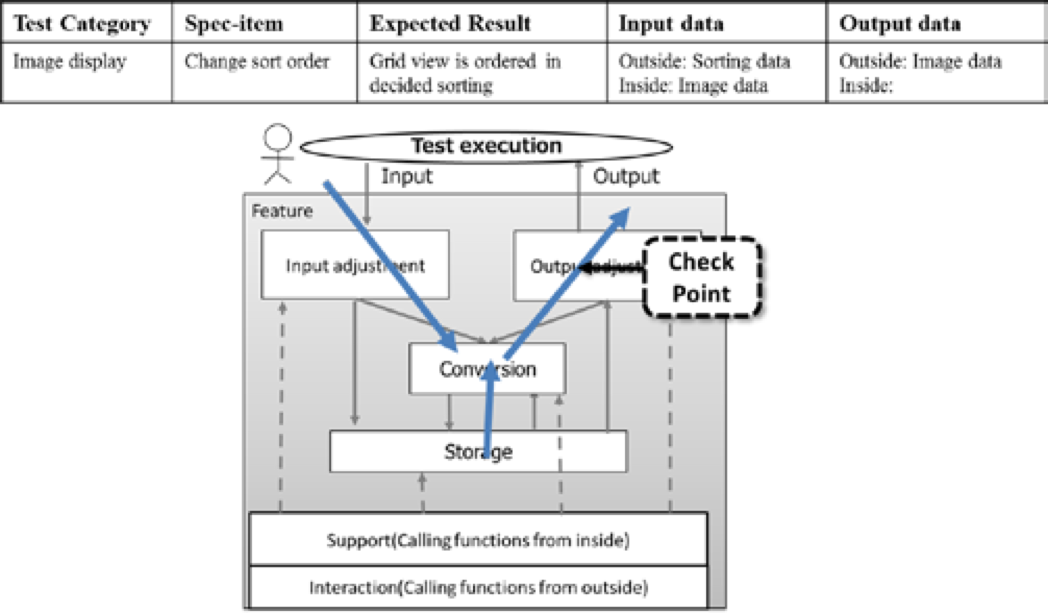
\includegraphics[width=10cm]{./image/D-4-Fig9.png}
\caption{仕様項目に入力データと出力データを加える方法の説明}
\label{fig:D-4-Fig9}
\end{center}
\end{figure}

\end{description}

\subsection{I/Oテストデータパターンを使ったテストベース分析}
I/Oテストデータパターンと既存のテスト分析手法であるテストカテゴリベースドテストを併用してテスト分析を行う.
作業ステップは以下のとおりである:
\begin{itemize}
 \item テストカテゴリを特定する.
 \item テストカテゴリ毎に入力データと出力データを明らかにする.
 \item I/Oテストデータパターンごとのデータフローをシミュレーションしてチェックポイント候補から仕様項目を選択する.
 \item 実プロジェクトのテストケースの分析結果をテストカテゴリに分類し,差異を比較する.
\end{itemize}

特定したテストカテゴリは,表~\ref{tab:D-4-TestCategory}のようになった.
サポートと相互作用については,テストカテゴリがトリガーとなる.トリガーから呼び出す$Ta$へのデータフローをシミュレーションして,仕様項目を特定した.


% Table generated by Excel2LaTeX from sheet 'Sheet2'修正
\begin{table}[htbp]
  \centering
  \caption{テストカテゴリ}
    \begin{tabular}{|l|p{5.415em}|l|l|l|l|}
    \hline
          \multicolumn{1}{|p{4em}|}{入力調整} & 出力調整 & \multicolumn{1}{p{2.5em}|}{変換} & \multicolumn{1}{p{3em}|}{貯蔵} & \multicolumn{1}{p{6em}|}{サポート} & \multicolumn{1}{p{6em}|}{相互作用} \bigstrut\\
    \hline
    \hline
\multicolumn{1}{|l|}{\multirow{3}[2]{*}{画面上操作}} & 画面表示  & \multicolumn{1}{l|}{\multirow{3}[2]{*}{計算}} & \multicolumn{1}{p{4em}|}{設定保存} & 割り込み  & リソース共有 \bigstrut[t]\\
                & メッセージ &       & \multicolumn{1}{p{4em}|}{画像保存} & 中断    & 反映 \\
                & 初期表示  &       &       & データ同時変更 & 並列処理 \bigstrut[b]\\
    \hline
    \end{tabular}%
  \label{tab:D-4-TestCategory}%
\end{table}%

\subsection{IOテストデータパターンの効果検証の結果}
テストカテゴリとI/Oテストデータパターンを使ったテストベースの分析で利用したI/Oテストデータパターンは表~\ref{tab:D-4-IOresult}のようになった.
実験に使ったフィーチャセットであるアップロードとグリッドビューの両方でテストカテゴリとI/Oテストデータパターンを使ったテストベースの分析が適用できた.
そして,両方のフィーチャセットにて,現実の開発で行われたシステムテストレベルのテストケースとI/Oテストデータパターンを使ったテスト分析結果を比較し,現実の開発で使われたテストケースに,テストすべき仕様項目が不足していることが実証できた.
分類に利用したI/Oテストデータパターンは,P5とP8を除く全てであった.

% Table generated by Excel2LaTeX from sheet 'Sheet3'
\begin{table}[htbp]
  \centering
  \caption{I/Oテストデータパターンの出現傾向}
    \begin{tabular}{|p{7em}|p{1.7em}|p{1.7em}|p{1.7em}|p{1.7em}|p{1.7em}|p{1.7em}|p{1.7em}|p{1.7em}|p{1.7em}|}
    \hline
    \multicolumn{1}{|r|}{} & \multicolumn{1}{l|}{P1} & \multicolumn{1}{l|}{P2} & \multicolumn{1}{l|}{P3} & \multicolumn{1}{l|}{P4} & \multicolumn{1}{l|}{P5} & \multicolumn{1}{l|}{P6} & \multicolumn{1}{l|}{P7} & \multicolumn{1}{l|}{P8} & \multicolumn{1}{l|}{P9} \bigstrut\\
    \hline
    \hline
    アップロード & ○     & ○     & ○     & ○     & X     & ○     & ○     & X     & ○ \bigstrut\\
    \hline
    グリッドビュー & ○     & X     & X     & ○     & X     & X     & ○     & X     & ○ \bigstrut\\
    \hline
    \end{tabular}%
  \label{tab:D-4-IOresult}%
\end{table}%

実プロジェクトのテスト条件との比較をした結果を図~\ref{fig:D-4-Fig10}に示す.
両者を比較すると,I/Oテストデータパターンを利用したテスト分析の結果が実プロジェクトより多くのテスト条件を選択できたことが確認できている.

\begin{figure}[htbp]
\begin{center}
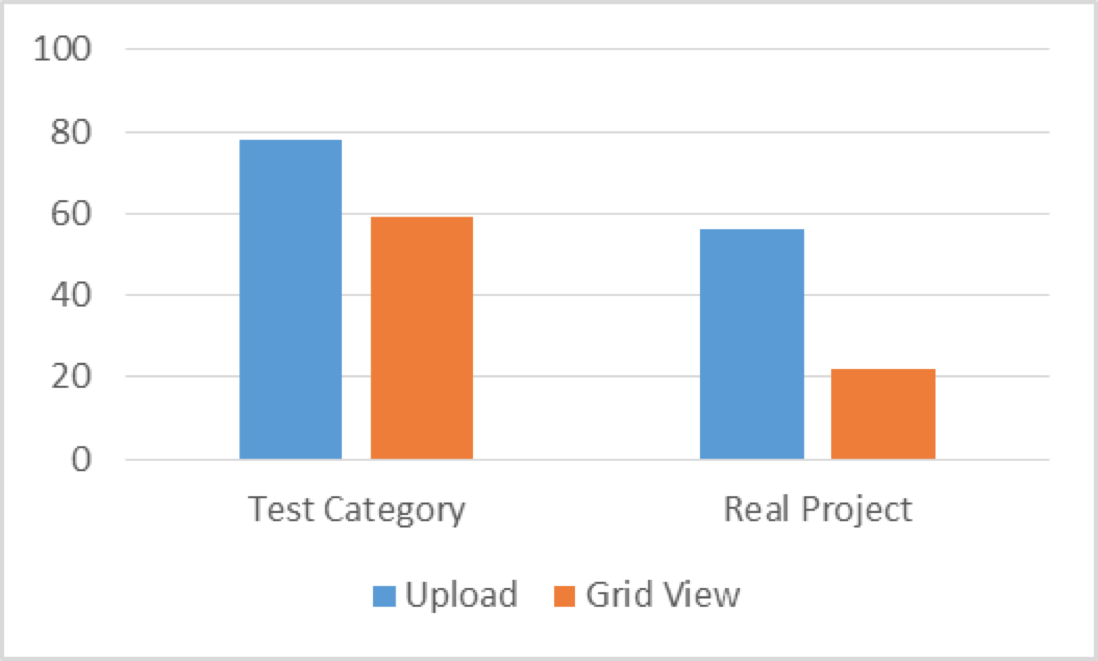
\includegraphics[width=12cm]{./image/D-4-Fig10.png}
\caption{実プロジェクトで特定したテスト条件の比較}
\label{fig:D-4-Fig10}
\end{center}
\end{figure}

\subsection{I/Oテストデータパターン毎の出現傾向の評価}
実プロジェクトで作られたテストケースとI/Oテストデータパターンを使ってテストベースの分析して特定した仕様項目の特定数をP1からP9の分類で出現割合を比較した結果が,表~\ref{tab:D-4-IOtestcompare}である.
% Table generated by Excel2LaTeX from sheet '結果比較'
\begin{table}[htbp]
  \centering
  \caption{I/Oテストデータパターン毎の特定数比較}
    \begin{tabular}{rrrrrrrrr}
    \multicolumn{1}{l}{アップロード} &  &     &       &       &       &       &       &  \bigstrut[b]\\
    \hline
    \multicolumn{1}{|l|}{パターン} &\multicolumn{1}{|l|}{P1} & \multicolumn{1}{l|}{P2} & \multicolumn{1}{l|}{P3} & \multicolumn{1}{l|}{P4} & \multicolumn{1}{l|}{P6} & \multicolumn{1}{l|}{P7} & \multicolumn{1}{l|}{P9} & \multicolumn{1}{l|}{合計} \bigstrut\\
    \hline
    \hline
    \multicolumn{1}{|l|}{TCとI/O} &\multicolumn{1}{|r|}{24} & \multicolumn{1}{r|}{6} & \multicolumn{1}{r|}{12} & \multicolumn{1}{r|}{14} & \multicolumn{1}{r|}{3} & \multicolumn{1}{r|}{7} & \multicolumn{1}{r|}{12} & \multicolumn{1}{r|}{78} \bigstrut\\
    \hline
    \multicolumn{1}{|l|}{現実のPJ} &\multicolumn{1}{|r|}{17} & \multicolumn{1}{r|}{6} & \multicolumn{1}{r|}{10} & \multicolumn{1}{r|}{10} & \multicolumn{1}{r|}{3} & \multicolumn{1}{r|}{5} & \multicolumn{1}{r|}{8} & \multicolumn{1}{r|}{59} \bigstrut\\
    \hline
    &71\%  & 100\% & 83\%  & 71\%  & 100\% & 71\%  & 67\%  & 76\% \bigstrut[t]\\
          &       &       &       &       &       &       &  \\
    \multicolumn{1}{l}{グリッドビュー}  & &       &       &       &       &       &       &  \bigstrut[b]\\
    \hline
    \multicolumn{1}{|l|}{パターン} &\multicolumn{1}{|l|}{P1} & \multicolumn{1}{r|}{--} & \multicolumn{1}{r|}{--} & \multicolumn{1}{l|}{P4} & \multicolumn{1}{r|}{--} & \multicolumn{1}{l|}{P7} & \multicolumn{1}{l|}{P9} & \multicolumn{1}{l|}{合計} \bigstrut\\
    \hline
    \hline
    \multicolumn{1}{|l|}{TCとI/O} &\multicolumn{1}{|r|}{25} & \multicolumn{1}{r|}{--} & \multicolumn{1}{r|}{--} & \multicolumn{1}{r|}{13} & \multicolumn{1}{r|}{--} & \multicolumn{1}{r|}{14} & \multicolumn{1}{r|}{4} & \multicolumn{1}{r|}{56} \bigstrut\\
    \hline
    \multicolumn{1}{|l|}{現実のPJ} &\multicolumn{1}{|r|}{5} & \multicolumn{1}{r|}{--} & \multicolumn{1}{r|}{--} & \multicolumn{1}{r|}{5} & \multicolumn{1}{r|}{--} & \multicolumn{1}{r|}{8} & \multicolumn{1}{r|}{4} & \multicolumn{1}{r|}{22} \bigstrut\\
    \hline
    &20\%  &       &       & 38\%  &       & 57\%  & 100\% & 39\% \bigstrut[t]\\
    \end{tabular}%
  \label{tab:D-4-IOtestcompare}%
\end{table}%

上段のTCとIOは,テストカテゴリとI/Oテストデータパターンを使ってテスト条件を特定した数であり,下段の現実のPJは,現実のプロジェクトでのテスト条件数である.欄外に記載した割合は,上段の数を母数にした場合の下段の現実のプロジェクトのテスト条件数の割合である.
両方の結果を合計したグラフが図~\ref{fig:D-4-Fig11}である.
図~\ref{fig:D-4-Fig11}からは,現実のプロジェクトにて不足していたテスト条件には,I/Oテストデータパターン別にみるとP1が特にテストカテゴリと実プロジェクトの差異が大きいことがわかる.
P1 は外部からの入力を行い,外部に出力する最も単純なパターンであり,I/O テストデータパターンから見ても単純なことを確認するテスト条件が漏れている.

\begin{figure}[htbp]
\begin{center}
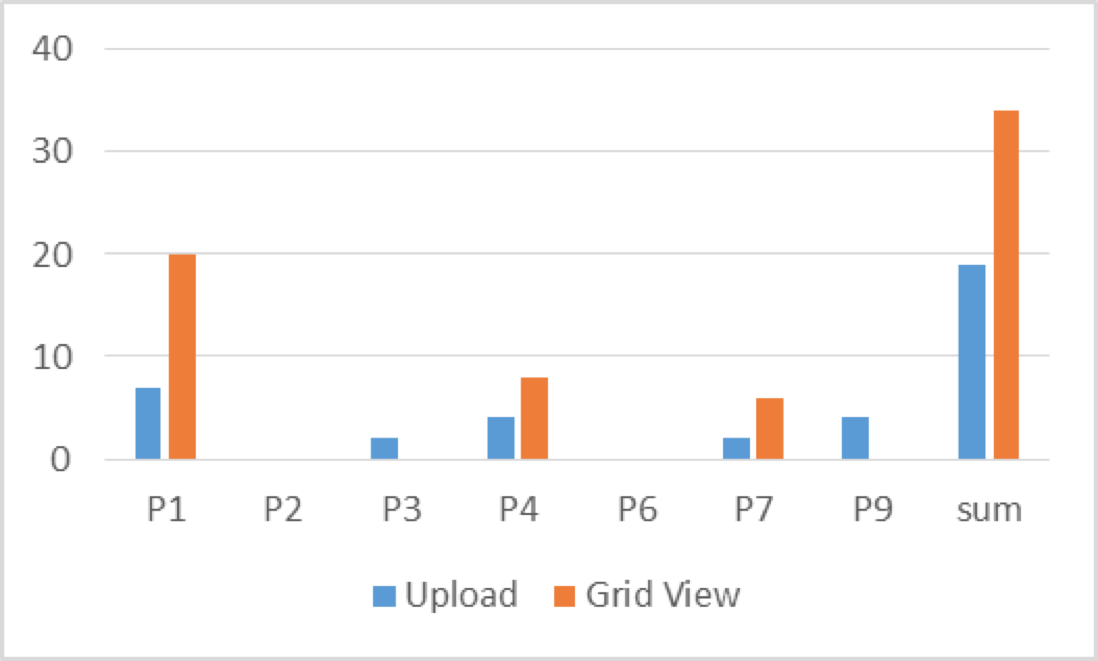
\includegraphics[width=12cm]{./image/D-4-Fig11.png}
\caption{IOテストデータパターンごとの違い}
\label{fig:D-4-Fig11}
\end{center}
\end{figure}

\subsection{I/Oテストデータパターンにて特定したテスト条件}
表~\ref{tab:D-4-ER-1}から表~\ref{tab:D-4-ER-4}に,I/Oテストデータパターンにて新たに特定したテスト条件となる仕様項目を全て列挙した.
これらのテスト条件は,全て今回のデータのI/Oのシミュレーションを行い網羅的にテストベースを確認することで特定できたものである.
I/Oテストデータパターンにて新たに特定したテスト条件には,論理的機能構造の要素別に見ると入力調整, 出力調整に分類できるテスト条件,例えばメッセージが現れることや入力制御といった単純な仕様項目でも漏れていることが確認できる.

一般的に,テスト条件となる仕様項目の一覧を作成せずに具体的なインスタンスとなるテストケースを列挙していく場合,テストパラメータ組み合わせの数量の多さに合わせてテストケースの数量が膨大になるため,網羅すべきテスト条件仕様項目の見易さが低下するため,仕様項目の数が不足することが多い.
実験結果も同様の傾向となった.

% Table generated by Excel2LaTeX from sheet 'Sheet2'
\begin{table}[htbp]
  \scriptsize
  \centering
  \caption{I/Oテストデータパターンにて特定したテスト条件(1/4)}
    \begin{tabular}{|p{8em}|p{7em}|p{9em}|p{9em}|p{3em}|p{12em}|}
\cline{1-6}   フィーチャセット & テストカテゴリ  & 仕様項目 & 期待結果  & I/O   & 入出力データ \bigstrut\\
    \hline
    \hline
    アップロード & データ同時変更 & アップロード中のアップロード済み画像のアルバム移動 & ロックがかかりできないこと & P9    & 外入:画像 内入:移動元画像
外出:件数 内出:画像 \bigstrut\\
    \hline
    アップロード & データ同時変更 & アップロード中のアップロード済み画像の情報変更 & ロックがかかりできないこと & P9    & 外入:情報 内入:画像情報
外出:変情 内出:画像情報 \bigstrut\\
    \hline
    アップロード & データ同時変更 & アップロード中のアップロード先アルバム名変更 & ロックがかかりできないこと & P9    & 外入:画像,アルバム名 内入:元アルバム名
外出:件数 内出:画像 \bigstrut\\
    \hline
    アップロード & データ同時変更 & アップロード中のアップロード前画像のアルバム移動 & ロックがかかりできないこと & P9    & 外入:画像 内入:移動元画像
外出:件数 内出:画像 \bigstrut\\
    \hline
    アップロード & メッセージ & 「画像を選択」時の選択枚数表示 & 「○枚の画像を選択中」というメッセージが出るか & P1    & 外入:画像選択 内入:--
外出:メッセージ 内出:-- \bigstrut\\
    \hline
    アップロード & メッセージ & 重複画像だけでアップロードした際の画像のアップロード & 「アップロードできない」というメッセージがでるか? & P1    & 外入:画像選択 内入:--
外出:メッセージ 内出:-- \bigstrut\\
    \hline
    アップロード & メッセージ & 「画像を選択」画面初期表示 & 「画像を選択」と表記が出ること & P1    & 外入:文字 内入:--
外出:文字 内出:-- \bigstrut\\
    \hline
    アップロード & メッセージ & 「画像を選択」時の選択枚数表示にて,選択済みの画像を押下 & 「○枚の画像を選択」というメッセージの枚数が減ること & P1    & 外入:画像選択 内入:--
外出:メッセージ 内出:-- \bigstrut\\
    \hline
    アップロード & メッセージ & 「画像を選択」時の選択枚数表示にて,選択済みの画像を押下 & 選択数が0になった場合,「画像を選択」と表記が出ること & P1    & 外入:画像選択 内入:--
外出:メッセージ 内出:-- \bigstrut\\
    \hline
    アップロード & 画像表示  & \multicolumn{1}{p{7.5em}|}{「アルバムに追加」でのアルバム一覧} & アルバム一覧の表示順が正しいこと & P4    & 外入:-- 内入:画像サムネイル,アルバム名
外出:画像サムネイル,アルバム名 内出:-- \bigstrut\\
    \hline
    アップロード & 画像表示  & \multicolumn{1}{p{7.5em}|}{「画像を選択」時の画像表示順} & 撮影日昇順で表示されること & p4    & 外入:-- 内入:画像
外出:画像 内出:-- \bigstrut\\
    \hline
    アップロード & 初期表示  & \multicolumn{1}{p{7.5em}|}{「アップロード」画面の操作} & 新規アルバムYYYY/MM/DDというアルバム名が表示されること & P4    & 外入:-- 内入:初期設定
外出:アルバム名 内出:-- \bigstrut\\
    \hline
    アップロード & 初期表示  & \multicolumn{1}{p{7.5em}|}{「アップロード」画面の操作} & 「すでにアップロード済みの画像を保存しない」がONになっていること & P4    & 外入:-- 内入:初期設定
外出:設定 内出:-- \bigstrut\\
    \hline
    アップロード & 画面上操作 & \multicolumn{1}{p{7.5em}|}{「アップロード」画面の操作} & 「すでにアップロード済みの画像を保存しない」がON→OFF→ONに変更できること & P1    & 外入:設定入力 内入:--
外出:設定 内出:-- \bigstrut\\
    \hline
    \end{tabular}%
  \label{tab:D-4-ER-1}%
\end{table}%

% Table generated by Excel2LaTeX from sheet 'Sheet4'
\begin{table}[htbp]

  \scriptsize
  \centering
  \caption{I/Oテストデータパターンにて特定したテスト条件(2/4)}
  \begin{tabular}{|p{8em}|p{7em}|p{9em}|p{9em}|p{3em}|p{12em}|}
\cline{1-6}   フィーチャセット & テストカテゴリ  & 仕様項目 & 期待結果  & I/O   & 入出力データ \bigstrut\\
    \hline
    \hline
    アップロード & 画面上操作 & \multicolumn{1}{p{7.5em}|}{「アルバムに追加」に表示されるアルバム名} & 「全画像」を選択できること & P7    & 外入:操作入力 内入:登録済画像
外出:登録済画像 内出:-- \bigstrut\\
    \hline
    アップロード & 画面上操作 & 「画像を選択」での画像選択 & 画像にタップするとチェックがつくこと & P7    & 外入:選択 内入:画像
外出:チェックアイコン 内出:-- \bigstrut\\
    \hline
    アップロード & 中断    & \multicolumn{1}{p{7.5em}|}{ネットワーク切断から再開したときのアップロード} & 一定以上の時間が過ぎるとアップロードが再開しない(要確認) & P1    & 外入:画像 内入:--
外出: メッセージ 内出:-- \bigstrut\\
    \hline
    アップロード & 画像保存  & \multicolumn{1}{p{7.5em}|}{アルバムの枚数が200枚以上になる枚数で画像を選択してアップロードのエラーが出た後に別のアルバムを選択してアップロード} & アップロードできた画像がNISにて表示できること & P3    & 外入:画像 内入:--
外出:枚数 内出:画像 \bigstrut\\
    \hline
    アップロード & 画像保存 & \multicolumn{1}{p{7.5em}|}{アップロードした画像の画質} & アップロードした画像が崩れていないこと & P3    & 外入:画像 内入:--
外出:枚数 内出:画像 \bigstrut\\
    \hline
    グリッドビュー & メッセージ & 選択画面初期表示 & 「画像を選択」と表記が出ること & P1    & 入力:文字
出力:文字 \bigstrut\\
    \hline
    グリッドビュー & メッセージ & 選択解除ボタン押下 & 「画像を選択」と表記が出ること & P1    & 入力:選択 文字
出力:文字 \bigstrut\\
    \hline
    グリッドビュー & メッセージ & \multicolumn{1}{p{7.5em}|}{選択済みの画像を押下} & 「○枚の画像を選択」というメッセージの枚数が減ること & P1    & 入力:選択
出力:文字 \bigstrut\\
    \hline
    グリッドビュー & メッセージ & \multicolumn{1}{p{7.5em}|}{選択済みの画像を押下} & 選択数が0になった場合,「画像を選択」と表記が出ること & P1    & 入力:選択
出力:文字 \bigstrut\\
    \hline
    グリッドビュー & メッセージ & 全て選択ボタン押下 & 「アルバムを選択中」というメッセージが出ること & P1    & 入力:選択
出力:文字 \bigstrut\\
    \hline
    グリッドビュー & メッセージ & 未選択の画像を押下 & 「○枚の画像を選択」というメッセージが出ること & P1    & 入力:選択
出力:文字 \bigstrut\\
    \hline
    グリッドビュー & 画像表示  & 1画面あたりの表示ファイル数 & 縦:4×10.横:3×7になること & P4    & 入力:既存設定
出力:文字 画像 \bigstrut\\
    \hline
    \end{tabular}%
  \label{tab:D-4-ER-2}%
\end{table}%

% Table generated by Excel2LaTeX from sheet 'Sheet4'
\begin{table}[htbp]
  \scriptsize
  \centering
  \caption{I/Oテストデータパターンにて特定したテスト条件(3/4)}
  \begin{tabular}{|p{8em}|p{7em}|p{9em}|p{9em}|p{3em}|p{12em}|}
\cline{1-6}   フィーチャセット & テストカテゴリ  & 仕様項目 & 期待結果  & I/O   & 入出力データ \bigstrut\\
    \hline
    \hline
    グリッドビュー & 画像表示  & スクロール時の枚数表示 & 複数ページのスクロールでファイルの日付と,現在の枚数順/全体の枚数が画面中央に表示されること & p7    & 入力:スクロール
出力:文字 画像 \bigstrut\\
    \hline
    グリッドビュー & 画像表示  & 画像ファイルの並び順 & 左から右方向に埋まっていくこと。 & P4    & 入力:既存設定
出力:文字 画像 \bigstrut\\
    \hline
    グリッドビュー & 画像表示  & 画像ファイルの並び順 & 2行目になるとまた左から埋まること & P4    & 入力:既存設定
出力:文字 画像 \bigstrut\\
    \hline
    グリッドビュー & 画像表示  & 更新ボタン押下 & 別デバイスで新しい画像の追加,名称の変更などをしていた場合,変更した画像に更新されること & P4    & 入力:既存設定
出力:画像 \bigstrut\\
    \hline
    グリッドビュー & 共有    & 他ビューの並び順影響有無 & 他のアルバムやビューで設定した並び順の影響を受けないこと & p4    & 入力:既存設定
出力:画像 \bigstrut\\
    \hline
    グリッドビュー & 設定保存  & 画面の並び順設定用画面 & 前回選択した並び順にチェックがついていること & p7    & 入力:並び順
出力:並び順 \bigstrut\\
    \hline
    グリッドビュー & 設定保存  & 画面の並び順設定用画面 & デフォルトでチェックされていること & p7    & 入力:並び順
出力:並び順 \bigstrut\\
    \hline
    グリッドビュー & 画面上操作 & OKボタン押下 & 全画像,カテゴリから移動したグリッドビューの場合のみOKボタンが現れ,共有設定画面に遷移する & P1    & 入力:既存設定
出力:画像 \bigstrut\\
    \hline
    グリッドビュー & 画面上操作 & \multicolumn{1}{p{7.5em}|}{アルバム追加ボタン押下} & アルバムから移動したグリッドビューの場合,アルバム追加画面に遷移する & P1    & 入力:既存設定
出力:文字 画像 \bigstrut\\
    \hline
    グリッドビュー & 画面上操作 & ダウンロードボタン押下 & アルバムから移動したグリッドビューの場合,DLサイズ選択画面に遷移する & P1    & 入力:既存設定
出力:文字 \bigstrut\\
    \hline
    グリッドビュー & 画面上操作 & 削除ボタン押下 & アルバムから移動したグリッドビューの場合,削除画面に遷移 & P1    & 入力:既存設定
出力:文字 \bigstrut\\
    \hline
    \multicolumn{1}{|l|}{グリッドビュー} & 画面上操作 & 選択画面初期表示 & 全画像から遷移したグリッドビューの場合,選択,解除,削除,アルバム追加,DLボタン出ない.OKボタン出る. & P1    & 入力:既存設定
出力:文字 画像 \bigstrut\\
    \hline
    \multicolumn{1}{|l|}{グリッドビュー} & 画面上操作 & 選択画面初期表示 & カテゴリから遷移したグリッドビューの場合,全画像からの遷移と同じであり,かつカテゴリを選択する選択用ビューがグレーアウトする & P1    & 入力:既存設定
出力:文字 画像 \bigstrut\\
    \hline
    \end{tabular}%
  \label{tab:D-4-ER-3}%
\end{table}%

% Table generated by Excel2LaTeX from sheet 'Sheet4'
    \begin{table}[htbp]
      \scriptsize
      \centering
      \caption{I/Oテストデータパターンにて特定したテスト条件(4/4)}
      \begin{tabular}{|p{8em}|p{7em}|p{9em}|p{9em}|p{3em}|p{12em}|}
    \cline{1-6}   フィーチャセット & テストカテゴリ  & 仕様項目 & 期待結果  & I/O   & 入出力データ \bigstrut\\
    \hline
    \hline
    \multicolumn{1}{|l|}{グリッドビュー} & 画面上操作 & 選択画面初期表示 & 端末の写真のグリッドビューの場合,最初から選択画面となり,チェックをすることでOKボタンが有効になる & P1    & 入力:既存設定
出力:文字 画像 \bigstrut\\
    \hline
    \multicolumn{1}{|l|}{グリッドビュー} & 画面上操作 & 選択解除ボタン押下 & 画面上の全ての画像のチェックが外れること & p1    & 入力:選択
出力:アイコン \bigstrut\\
    \hline
    \multicolumn{1}{|l|}{グリッドビュー} & 画面上操作 & \multicolumn{1}{p{7.5em}|}{選択済みの画像を押下} & 画像のチェックが外れること & p1    & 入力:選択
出力:アイコン \bigstrut\\
    \hline
    \multicolumn{1}{|l|}{グリッドビュー} & 画面上操作 & 全て選択ボタン押下 & 画面上の全ての画像にチェックがつくこと & p1    & 入力:選択
出力:アイコン \bigstrut\\
    \hline
    \multicolumn{1}{|l|}{グリッドビュー} & 画面上操作 & 未選択の画像を押下 & 画像のチェックがつくこと & p1    & 入力:選択
出力:アイコン \bigstrut\\
    \hline
    \multicolumn{1}{|l|}{グリッドビュー} & 画面上操作 & 未選択の画像を押下 & 全てチェックの場合,押下した画像以外のチェックが全て外れること & p1    & 入力:選択
出力:アイコン \bigstrut\\
    \hline
    \multicolumn{1}{|l|}{グリッドビュー} & 画面上操作 & フロービューボタン押下 & フロービューに遷移すること & P7    & 入力:既存設定
出力:文字 画像 \bigstrut\\
    \hline
    \multicolumn{1}{|l|}{グリッドビュー} & 画面上操作 & マップビュー押下 & マップビューに遷移すること & P7    & 入力:既存設定
出力:文字 画像 \bigstrut\\
    \hline
    \multicolumn{1}{|l|}{グリッドビュー} & 画面上操作 & 画像選択ボタン押下 & ピクチャービューに遷移すること & P7    & 入力:既存設定
出力:文字 画像 \bigstrut\\
    \hline
    \multicolumn{1}{|l|}{グリッドビュー} & 画面上操作 & 画面の並び順設定用画面 & ファイル名,アップロード名,撮影日,ファイルサイズ,ファイル形式,お気に入り,マイルールの順で一覧表示されていること & P1    & 入力:既存設定
出力:文字 \bigstrut\\
    \hline
    \multicolumn{1}{|l|}{グリッドビュー} & 画面上操作 & 並び順の変更 & 一覧項目の横をタップするとチェックがつくこと & p1    & 入力:設定
出力:設定 \bigstrut\\
    \hline
    グリッドビュー & 中断    & ネットワーク切断時のグリッドビュー初期表示 & キャッシュがある場合,キャッシュされた画像が一覧表示されること & P4    & 入力:既存設定
出力:文字 画像 \bigstrut\\
    \hline
    グリッドビュー & 中断    & ネットワーク切断時のグリッドビュー初期表示 & キャッシュの限界を超えた場合,その画像が一覧表示されないこと & P4    & 入力:既存設定
出力:文字 画像 \bigstrut\\
    \hline
    グリッドビュー & 中断    & ネットワーク切断時の更新ボタン押下 & キャッシュがある場合,更新ボタンを押すと別デバイスの変更が反映されず画像が表示される & P4    & 入力:既存設定
出力:文字 画像 \bigstrut\\
    \hline
    \end{tabular}%
    \label{tab:D-4-ER-4}%
  \end{table}%

  \newpage
  \section{まとめ}
  本章では,テスト実行時のデータ入出力の要素で分類し網羅的に分析するI/Oテストデータパターンを提案した.そして,入手した現実の開発プロジェクトのテストケースを使い,I/Oテストデータパターンで特定したテスト条件との比較を試みた.
  提案したI/Oテストデータパターンで特定したテスト条件と実プロジェクトで作られるテストケースと比較して,不足しているテスト条件の発見が可能であることが確認できた.

  また,実プロジェクトで作られたテストケースからまとめ直したテスト条件の一覧を表~\ref{tab:D-4-ER2-1}から表~\ref{tab:D-4-ER2-6}に列挙した.
  これらのテスト条件はI/Oテストデータパターンを使ったシミュレーションでも全て特定可能であった.


  \begin{table}[htbp]
    \scriptsize
    \centering
    \caption{実プロジェクトのテストで使われたテスト条件(1/6)}
    \begin{tabular}{|p{8em}|p{7em}|p{9em}|p{9em}|p{3em}|p{12em}|}
  \cline{1-6}   フィーチャセット & テストカテゴリ  & 仕様項目 & 期待結果  & I/O   & 入出力データ \bigstrut\\
      \hline
      \hline
    アップロード & データ同時変更 & アップロード先のアルバムに複数のデバイスからアップロードして結果的に合計が200枚以上になる枚数で画像を選択してアップロード & (要確認) & P3    & 外入:画像 内入:---
外出:件数 内出:画像 \bigstrut\\
    \hline
    アップロード & データ同時変更 & アップロード中のアップロード済み画像が入るアルバム削除 & 未整理の画像としてアップロードされる?(要確認) & P9    & 外入:画像 内入:元アルバム名
外出:件数 内出:画像 \bigstrut\\
    \hline
    アップロード & データ同時変更 & アップロード中のアップロード済み画像の削除 & (要確認) & P9    & 外入:画像 内入:削除元画像
外出:件数 内出:画像 \bigstrut\\
    \hline
    アップロード & データ同時変更 & アップロード中のアップロード前画像の削除 & (要確認) & P9    & 外入:画像 内入:削除元画像
外出:件数 内出:画像 \bigstrut\\
    \hline
    アップロード & データ同時変更 & アップロード中のアップロード前画像の情報変更 & (要確認) & P9    & 外入:情報 内入:画像情報
外出:変情 内出:画像情報 \bigstrut\\
    \hline
    アップロード & メッセージ & 100枚以上の画像を選択してアップロード & 「規定以上の枚数はアップロードできない」というメッセージが出て処理が終了する & P3    & 外入:画像選択,画像 内入:--
外出:件数 内出:画像 \bigstrut\\
    \hline
    アップロード & メッセージ & アップロード先のアルバムの枚数が200枚以上になる枚数で画像を選択してアップロード & 「規定以上の枚数はアップロードできない」というメッセージ出てが出て処理が終了する & P1    & 外入:画像選択 内入:--
外出:メッセージ 内出:-- \bigstrut\\
    \hline
    アップロード & メッセージ & マイフォト全体での枚数のMAXを超えたときの画像のアップロード & 画像が上限に達したことを知らせるメッセージが出て処理が終了する & P1    & 外入:画像選択 内入:--
外出:メッセージ 内出:-- \bigstrut\\
    \hline
    アップロード & メッセージ & アルバム数がMAX(3500)を超えたときの新規アルバム追加のアップロード & アルバムが上限に達したことを知らせるメッセージが出て処理が終了する & P1    & 外入:画像選択 内入:--
外出:メッセージ 内出:-- \bigstrut\\
    \hline
    アップロード & メッセージ & アップロード終了時のDL/UL一覧へのメッセージ & DL/UL一覧で終了したことがわかること & P1    & 外入:画像 内入:--
外出:メッセージ 内出:-- \bigstrut\\
    \hline
    アップロード & 画像表示  & アップロードした画像の表示確認 & 画像にアップロードアイコンが付与されて表示されている & p4    & 外入:-- 内入:画像
外出:画像 内出:-- \bigstrut\\
    \hline
    アップロード & 画像表示  & 「アルバムに追加」でのアルバム一覧 & アルバムが無い場合はアルバムが出てこないこと & P4    & 外入:-- 内入:画像サムネイル,アルバム名
外出:画像サムネイル,アルバム名 内出:-- \bigstrut\\
    \hline
    アップロード & 画像表示  & 「画像を選択」で表示される画像種類 & 動画(アップロードできないコンテンツ)が選択画面に出てこないこと & P4    & 外入:-- 内入:画像
外出:画像 内出:-- \bigstrut\\
    \hline
    アップロード & 画像表示  & 「画像を選択」時の画像表示 & 複数ページにまたがる場合はスクロールできること & p7    & 外入:フリック 内入:画像
外出:画像 内出:-- \bigstrut\\
    \hline
    \end{tabular}%
  \label{tab:D-4-ER2-1}%
\end{table}%


\begin{table}[htbp]
  \scriptsize
  \centering
  \caption{実プロジェクトのテストで使われたテスト条件(2/6)}
  \begin{tabular}{|p{8em}|p{7em}|p{9em}|p{9em}|p{3em}|p{12em}|}
\cline{1-6}   フィーチャセット & テストカテゴリ  & 仕様項目 & 期待結果  & I/O   & 入出力データ \bigstrut\\
    \hline
    \hline
    アップロード & 画像表示  & \multicolumn{1}{p{8em}|}{アップロード状況確認画面} & アップロードできた画像が先に表示されこれからアップロードする画像が色が黒っぽく表示されること & P9    & 外入:画像 内入:登録済画像
外出:画像登録結果 内出:画像 \bigstrut\\
    \hline
    アップロード & 画像表示  & \multicolumn{1}{p{8em}|}{アップロード状況確認画面} & ドラッグ&ドロップでアップロード済とアップロード前の画像の表示を入れ替えることができないこと & P7    & 外入:操作入力 内入:画像
外出:表示位置 内出:-- \bigstrut\\
    \hline
    アップロード & 画像表示  & \multicolumn{1}{p{8em}|}{アップロード状況確認画面} & 複数ページにまたがる場合はスクロールできること & p7    & 外入:フリック 内入:画像
外出:画像 内出:-- \bigstrut\\
    \hline
    アップロード & 画像保存  & \multicolumn{1}{p{8em}|}{画像のアップロード実施} & アップロードできた画像がNISにて表示できること & P2    & 外入:画像 内入:--
外出:-- 内出:画像 \bigstrut\\
    \hline
    アップロード & 画像保存  & \multicolumn{1}{p{8em}|}{画像のアップロード実施} & JPGとして保存されること & P2    & 外入:画像 内入:--
外出:-- 内出:画像 \bigstrut\\
    \hline
    アップロード & 画像保存  & \multicolumn{1}{p{8em}|}{重複画像のアップロード無効} & 重複画像がアップロードされていないこと & P2    & 外入:画像(なし) 内入:--
外出:-- 内出:画像(なし) \bigstrut\\
    \hline
    アップロード & 画像保存  & \multicolumn{1}{p{8em}|}{アップロード画像の名称がMAXを超える} & 要確認??? & P2    & 外入:画像(なし) 内入:--
外出:-- 内出:画像(なし) \bigstrut\\
    \hline
    アップロード & 割り込み  & \multicolumn{1}{p{8em}|}{アップロード中に電話などの割り込み入る} & 処理は継続する(要確認) & P3    & 割り込みで処理をバックグランドにするタスクだが,I/Oとしてはその間P3が続いている
外入:画像 内入:--
外出:枚数 内出:画像 \bigstrut\\
    \hline
    アップロード & 計算    & \multicolumn{1}{p{8em}|}{アップロード中のDL/UL一覧} & DL/UL一覧で何枚までアップロードしているかがわかること & P3    & 外入:画像 内入:--
外出:枚数 内出:画像 \bigstrut\\
    \hline
    アップロード & 画面上操作 & \multicolumn{1}{p{8em}|}{「アルバム名編集」でのアルバム名が空白} & アルバム名の保存ボタンが押下ができないこと & P1    & 外入:設定入力 内入:--
外出:設定 内出:-- \bigstrut\\
    \hline
    アップロード & 画面上操作 & \multicolumn{1}{p{8em}|}{「アルバム名編集」でのアルバム名が空白} & 40文字を超えて入力できないこと & P1    & 外入:設定入力 内入:--
外出:設定 内出:-- \bigstrut\\
    \hline
    アップロード & 画面上操作 & \multicolumn{1}{p{8em}|}{「アルバムに追加」でのアルバム名変更} & 新規アルバム名変更でアルバム名が変更できること & P1    & 外入:アルバム名入力 内入:--
外出:アルバム名 内出:-- \bigstrut\\
    \hline
    アップロード & 画面上操作 & \multicolumn{1}{p{8em}|}{「アルバムに追加」に表示されるアルバム名} & 既存のアルバムを選択できること & P1    & 外入:-- 内入:アルバム名
外出:アルバム名 内出:-- \bigstrut\\
    \hline
    アップロード & 画面上操作 & 「画像を選択」での画像選択 & ドラッグによる表示順移動ができないこと & P7    & 外入:操作入力 内入:画像
外出:表示位置 内出:-- \bigstrut\\
    \hline
    アップロード & 画面上操作 & 「画像を選択」でのアップロードボタン押下 & DL/ULアイコンが表示されもとの画面にもどること & P3    & 外入:選択,画像 内入:--
外出:枚数 内出:画像 \bigstrut\\
    \hline
    \end{tabular}%
  \label{tab:D-4-ER2-2}%
\end{table}%

\begin{table}[htbp]
  \scriptsize
  \centering
  \caption{実プロジェクトのテストで使われたテスト条件(3/6)}
  \begin{tabular}{|p{8em}|p{7em}|p{9em}|p{9em}|p{3em}|p{12em}|}
\cline{1-6}   フィーチャセット & テストカテゴリ  & 仕様項目 & 期待結果  & I/O   & 入出力データ \bigstrut\\
    \hline
    \hline
    アップロード & 画面上操作 & 「画像を選択」でのアップロードボタン押下 & 画像が選択されていないときにはアップロード画面へ遷移しないこと & P1    & 外入:選択 内入:--
外出: メッセージ 内出:-- \bigstrut\\
    \hline
    アップロード & 画面上操作 & DL/UL一覧のXボタン押下 & キャンセルダイアログに遷移すること & P1    & 外入:選択 内入:---
外出: メッセージ 内出:--- \bigstrut\\
    \hline
    アップロード & 画面上操作 & DL/UL一覧の件数 & DL/UL一覧が20件を超えると古いものから削除されること & P1    & 外入:選択 内入:--
外出: メッセージ 内出:-- \bigstrut\\
    \hline
    アップロード & 画面上操作 & DL/UL中に新規にアップロードを行う & Waiting状態になり,前の処理が終了するとアップロードを開始すること & P3    & 外入:選択 画像 内入:--
外出: メッセージ 内出:画像 \bigstrut\\
    \hline
    アップロード & 画面上操作 & DL/ULアイコンからの遷移 & DL/UL一覧へ遷移すること & P3    & 外入:選択 画像 内入:--
外出: 登録済み件数 内出:画像 \bigstrut\\
    \hline
    アップロード & 画面上操作 & DL/UL一覧でUL中を選択 & 状況確認画面へ遷移する & P9    & 外入:選択 画像 内入:登録済画像情報
外出: 登録済み件数 内出:画像 \bigstrut\\
    \hline
    アップロード & 画面上操作 & DL/UL一覧でのクローズボタン押下 & DL/ULアイコンに戻る。遷移先画面は遷移元画面と同じであること。 & P3    & 外入:選択 画像 内入:--
外出: アイコン 内出:画像 \bigstrut\\
    \hline
    アップロード & 画面上操作 & キャンセル実行 & DL/UL一覧にてキャンセルボタンが出てこなくなること。 & P1    & 外入:選択 内入:--
外出: 表示 内出:-- \bigstrut\\
    \hline
    アップロード & 中断    & アップロードのネットワーク切断 & アップロードが止まる(要確認) & P1    & 外入:止めるための情報 画像 内入:--
外出: メッセージ 内出:-- \bigstrut\\
    \hline
    アップロード & 中断    & ネットワーク切断から再開したときのアップロード & 中断していたアップロードが再開すること。 & P3    & 外入:画像 内入:--
外出: 件数 内出:画像 \bigstrut\\
    \hline
    アップロード & 中断    & アップロード中にアプリからログアウトした際のアップロード & アップロードを継続するか?(要確認) & P2    & 外入:画像 内入:--
外出: ーー 内出:画像 \bigstrut\\
    \hline
    アップロード & 中断    & キャンセル時のアップロード画像の扱い & キャンセルするまでの画像がアップロードできて,その後の画像はアップロードしていないこと & P1    & 外入:選択 内入:--
外出: 表示 内出:-- \bigstrut\\
    \hline
    アップロード & 中断    & アップロード中にアプリからログアウトした際のDL/UL一覧 & DL/UL一覧が全てクリアされる & P1    & 外入:選択 内入:--
外出: 表示 内出:-- \bigstrut\\
    \hline
    アップロード & 中断    & アップロード中にアプリを終了した際のDL/UL一覧 & DL/UL一覧が全てクリアされる & P1    & 外入:選択 内入:--
外出: 表示 内出:-- \bigstrut\\
    \hline
    アップロード & 中断    & アップロード中にアプリを終了した際のアップロード & 中断する(要確認) & P1    & 外入:選択 内入:--
外出: 表示 内出:-- \bigstrut\\
    \hline
    アップロード & 中断    & アップロード中にデバイスの電源を切った際のDL/UL一覧 & DL/UL一覧が全てクリアされる & P1    & 外入:選択 内入:--
外出: 表示 内出:-- \bigstrut\\
    \hline
    \end{tabular}%
  \label{tab:D-4-ER2-3}%
\end{table}%


\begin{table}[htbp]
  \scriptsize
  \centering
  \caption{実プロジェクトのテストで使われたテスト条件(4/6)}
  \begin{tabular}{|p{8em}|p{7em}|p{9em}|p{9em}|p{3em}|p{12em}|}
\cline{1-6}   フィーチャセット & テストカテゴリ  & 仕様項目 & 期待結果  & I/O   & 入出力データ \bigstrut\\
    \hline
    \hline
    アップロード & 反映    & アップロードした画像の詳細情報 & 位置情報など全部の情報が登録されていること & P4    & 外入:-- 内入:画像
外出: 画像 内出:-- \bigstrut\\
    \hline
    アップロード & 反映    & アップロードした画像の場所 & 指定したアルバムの中にだけ表示されていること & P4    & 外入:-- 内入:画像
外出: 画像 内出:-- \bigstrut\\
    \hline
    アップロード & 反映    & アップロードした画像の表示 & 各種ビューでバリエーションとして確認 & P4    & 外入:-- 内入:画像
外出: 画像 内出:-- \bigstrut\\
    \hline
    アップロード & 反映    & アップロード中画像のダウンロード & ダウンロードができること & P4    & 外入:-- 内入:画像
外出: 画像,枚数 内出:-- \bigstrut\\
    \hline
    アップロード & 反映    & アップロードした際に作成したアルバム確認 & マイフォトにてアルバムが出来ていること & P4    & 外入:-- 内入:アルバム
外出: アルバム,枚数 内出:-- \bigstrut\\
    \hline
    アップロード & 並列処理  & アップロード中に共有フォルダを作成する & 影響を与えないでアップロードが続く & P3    & 割り込みで処理をバックグランドにするタスクだが,I/Oとしてはその間P3が続いている
外入:画像 内入:--
外出:枚数 内出:画像 \bigstrut\\
    \hline
    アップロード & 並列処理  & アップロード中に設定画面へ遷移し操作する & 設定をしている間もアップロードが続くこと & P3    & 割り込みで処理をバックグランドにするタスクだが,I/Oとしてはその間P3が続いている
外入:画像 内入:--
外出:枚数 内出:画像 \bigstrut\\
    \hline
    アップロード & 並列処理  & アップロード中に他のビューで閲覧する & 各種ビューでバリエーションとして確認 & P7    & 割り込みで処理をバックグランドにするタスクだが,I/Oとしてはその間P3が続いている
外入:選択 内入:画像
外出:画像 内出:-- \bigstrut\\
    \hline
    アップロード & 並列処理  & アップロード中に他のビューで閲覧する & 閲覧中もアップロードが続く & P3    & 割り込みで処理をバックグランドにするタスクだが,I/Oとしてはその間P3が続いている
外入:画像 内入:--
外出:枚数 内出:画像 \bigstrut\\
    \hline
    アップロード & データ同時変更 & アップロード中のアップロード済み画像が入るアルバム削除 & アルバムを削除した後に同じアルバム名を作って再度アップロードを繰り返した際にアップロードができること & P9    & 外入:画像 内入:削除元画像
外出:件数 内出:画像 \bigstrut\\
    \hline
    アップロード & 画像保存  & アルバムの枚数が200枚以上になる枚数で画像を選択してアップロードのエラーが出た後に別のアルバムを選択してアップロード & アップロードした画像の詳細情報の登録ができていること & P2    & 入力:画像情報
出力:画像情報 \bigstrut\\
    \hline
    アップロード & 画像保存  & 一度アップロードした画像を削除してまた同じ画像をアップロードする & アップロードできた画像がNISにて表示できること & P3    & 外入:画像 内入:--
外出:枚数 内出:画像 \bigstrut\\
    \hline
    \end{tabular}%
  \label{tab:D-4-ER2-4}%
\end{table}%



\begin{table}[htbp]
  \scriptsize
  \centering
  \caption{実プロジェクトのテストで使われたテスト条件(5/6)}
  \begin{tabular}{|p{8em}|p{7em}|p{9em}|p{9em}|p{3em}|p{12em}|}
\cline{1-6}   フィーチャセット & テストカテゴリ  & 仕様項目 & 期待結果  & I/O   & 入出力データ \bigstrut\\
    \hline
    \hline
    アップロード & 画面上操作 & \multicolumn{1}{p{8em}|}{DL/UL中にダウンロードが失敗やキャンセルなど処理が中断した後に新規にアップロードを行う} & 直前のパターンが失敗する,キャンセルする,失敗が続く,エラーがでるといった状況を複数組み合わせてアップロード対象がアップロードできることを確認する & P3    & 外入:画像 内入:--
外出:枚数 内出:画像 \bigstrut\\
    \hline
    アップロード & 反映    & \multicolumn{1}{p{8em}|}{アップロード中画像がエラーになる場合のダウンロード} & エラーなったときのその直前の成功した画像,アップロードが失敗する画像のダウンロードができること & P4    & 外入:-- 内入:画像
外出: 画像,枚数 内出:-- \bigstrut\\
    \hline
    グリッドビュー & メッセージ & \multicolumn{1}{p{8em}|}{規定枚数以上の画像を押下} & 「一度に選択できる画像は100枚までです」というメッセージが出る & P1    & 入力:選択
出力:文字 \bigstrut\\
    \hline
    グリッドビュー & 画像表示  & デフォルトの画像ファイル表示順 & デフォルト設定にあわせて表示されること & P4    & 入力:既存設定
出力:文字 画像 \bigstrut\\
    \hline
    グリッドビュー & 画像表示  & デフォルトの画像レイアウト & 縦横が基の画像のとおりに表示されること & P4    & 入力:既存設定
出力:文字 画像 \bigstrut\\
    \hline
    グリッドビュー & 画像表示  & 画像枚数がゼロ & 空白で表示されること & P1    & 入力:既存設定
出力:文字 \bigstrut\\
    \hline
    グリッドビュー & 画像表示  & 並び順設定後の画像ファイル表示順 & ファイル名で表示されること(昇順,降順) & p7    & 入力:並び順
出力:文字 画像 \bigstrut\\
    \hline
    グリッドビュー & 画像表示  & 並び順設定後の画像ファイル表示順 & アップロード名の昇順で表示されること & p7    & 入力:並び順
出力:文字 画像 \bigstrut\\
    \hline
    グリッドビュー & 画像表示  & 並び順設定後の画像ファイル表示順 & 撮影日の昇順で表示されること & p7    & 入力:並び順
出力:文字 画像 \bigstrut\\
    \hline
    グリッドビュー & 画像表示  & 並び順設定後の画像ファイル表示順 & ファイルサイズの昇順で表示されること & p7    & 入力:並び順
出力:文字 画像 \bigstrut\\
    \hline
    グリッドビュー & 画像表示  & 並び順設定後の画像ファイル表示順 & ファイル形式の昇順で表示されること & p7    & 入力:並び順
出力:文字 画像 \bigstrut\\
    \hline
    グリッドビュー & 画像表示  & 並び順設定後の画像ファイル表示順 & お気に入りの昇順で表示されること & p7    & 入力:並び順
出力:文字 画像 \bigstrut\\
    \hline
    グリッドビュー & 画像表示  & 並び順設定後の画像ファイル表示順 & マイルールで設定した順番で表示されること & p7    & 入力:並び順
出力:文字 画像 \bigstrut\\
    \hline
    グリッドビュー & 画像表示  & 戻るボタン押下 & マイフォト画面に遷移すること & P4    & 入力:既存設定
出力:画像 \bigstrut\\
    \hline
    グリッドビュー & 設定保存  & ドラッグドロップによるマイルール作成 & ドラッグドロップの表示位置変更結果をマイルールとして保存すること & p9    & 入力:画像,並び順
出力:画像,マイルール \bigstrut\\
    \hline
    グリッドビュー & 画面上操作 & 選択画面初期表示 & 全て選択ボタン,選択解除ボタンの位置が上もしくは下のどちらかに現れること & P1    & 入力:既存設定
出力:文字 \bigstrut\\
    \hline
    グリッドビュー & 画面上操作 & 「並び順」ボタン押下 & 画像の並び順画面に遷移すること & p1    & 入力:既存設定
出力:並び順 \bigstrut\\
    \hline
    \end{tabular}%
  \label{tab:D-4-ER2-5}%
\end{table}%


\begin{table}[htbp]
  \scriptsize
  \centering
  \caption{実プロジェクトのテストで使われたテスト条件(6/6)}
  \begin{tabular}{|p{8em}|p{7em}|p{9em}|p{9em}|p{3em}|p{12em}|}
\cline{1-6}   フィーチャセット & テストカテゴリ  & 仕様項目 & 期待結果  & I/O   & 入出力データ \bigstrut\\
    \hline
    \hline
    \multicolumn{1}{|c|}{グリッドビュー} & 画面上操作 & スクロール & 上下にスクロールできること & p1    & 入力:選択
出力:表示 \bigstrut\\
    \hline
    \multicolumn{1}{|c|}{グリッドビュー} & 画面上操作 & ドラッグドロップによる表示位置変更 & ドラッグドロップした位置に移動できること & p9    & 入力:画像,並び順
出力:画像,マイルール \bigstrut\\
    \hline
    \multicolumn{1}{|c|}{グリッドビュー} & 画面上操作 & 画像押下  & ピクチャービューに遷移すること & P7    & 入力:既存設定
出力:文字 画像 \bigstrut\\
    \hline
    \multicolumn{1}{|c|}{グリッドビュー} & 画面上操作 & 並び順の変更 & 変更したい並び順を選択するとグリッドビュー画面に遷移すること & p9    & 入力:画像,並び順
出力:画像,並び順 \bigstrut\\
    \hline
    \multicolumn{1}{|c|}{グリッドビュー} & 画面上操作 & 並び順の変更 & 変更したソート順で表示されること & p9    & 入力:画像,並び順
出力:画像,並び順 \bigstrut\\
    \hline
    グリッドビュー & 中断    & ネットワーク切断時のグリッドビュー初期表示 & キャッシュがない場合,グリッドビューを表示すると画像が表示されないこと & P4    & 入力:既存設定
出力:画像(なし) \bigstrut\\
    \hline
    グリッドビュー & 中断    & ネットワーク切断時の更新ボタン押下 & キャッシュがない場合,更新ボタンを押すと「インターネット接続がオフラインのようです」のメッセージがでる & P4    & 入力:既存設定
出力:画像(なし) \bigstrut\\
    \hline
    \end{tabular}%
  \label{tab:D-4-ER2-6}%
\end{table}%
